\documentclass{article}
\usepackage{fullpage}
\usepackage{mathptmx}
%\usepackage{graphicx}
\usepackage{amsmath}
\usepackage{floatflt}
\usepackage[aux]{rerunfilecheck}
\usepackage{tikz}
\usetikzlibrary{calc}

\newcommand{\ds}{\displaystyle}

\title{MATH 110 Sample Final Exam 3 Solutions}
\author{Edward Doolittle}

\begin{document}
\maketitle

\begin{enumerate}
\item 
  \begin{enumerate}
  \item %1a
    Writing in power notation,
    \begin{equation*}
      y= x^{-1/3} - x^7 + \cos x
    \end{equation*}
    By the sum rule,
    \begin{equation*}
      \frac{dy}{dx} = \frac{dy}{dx} \left( x^{-1/3} - x^7 + \cos x\right)
      = \frac{d}{dx} x^{-1/3} - \frac{d}{dx} x^7 + \frac{d}{dx} \cos x
      = -\frac{1}{3} x^{-4/3} - 7 x^6 - \sin x
    \end{equation*}
    by the rules for differentiating powers and trig functions.
  \item %1b
    By the quotient rule,
    \begin{equation*}
      \frac{dy}{dx} = \frac{\left(\frac{d}{dx}\sin^2(3x)\right)(x^3-3)
      - \sin^2(3x) \left(\frac{d}{dx} (x^3-3)\right) }{(x^3-3)^2}
    \end{equation*}
    By the chain rule applied twice,
    \begin{equation*}
      \frac{d}{dx} \sin^2(3x)
      = \frac{d}{dx} (\sin(3x))^2
      = 2 \sin(3x) \frac{d}{dx} \sin(3x)
      = 2 \sin(3x) \cos(3x) \frac{d}{dx} (3x)
      = 6 \sin(3x)\cos(3x)
    \end{equation*}
    so the final answer is
    \begin{equation*}
      \frac{dy}{dx} = \frac{6\sin(3x)\cos(3x)(x^3-3)
      - \sin^2(3x) \cdot 3x^2}{(x^3-3)^2}
    \end{equation*}
    Some simplification may be possible but is not necessary.
  \item %1c
    Using implicit differentiation and the chain and product rules we have
    \begin{equation*}
      \frac{d}{dx} (2y^4+x^2+xy^2) = \frac{d}{dx} 4
      \implies 8y^3 \frac{dy}{dx} + 2x + y^2 + 2xy \frac{dy}{dx} = 0
    \end{equation*}
    Solving for $dy/dx$ we have
    \begin{equation*}
      (8y^3+2xy) \frac{dy}{dx} = -2x-y^2
      \implies \frac{dy}{dx} = -\frac{2x+y^2}{8y^3+2xy}
    \end{equation*}
  \item %1d
    By the Fundamental Theorem of Calculus part I we have
    \begin{equation*}
      \frac{dy}{dx} = \frac{d}{dx} \int_1^x \frac{\cos t}{t} \; dt
      = \frac{\cos x}{x}
    \end{equation*}
  \end{enumerate}
\item %2
  \begin{enumerate}
  \item %2a
    Multiplying and dividing by $3$ to make it look more like a basic trig
    limit,
    \begin{equation*}
      \lim_{x\to 0} \frac{\sin 3x}{2x}
      = \lim_{x\to 0} \frac{3}{2} \frac{\sin 3x}{3x}
      = \frac{3}{2} \lim_{x\to 0} \frac{\sin 3x}{3x}
      = \frac{3}{2} \cdot 1
    \end{equation*}
  \item %2b
    Multiplying out the denominator to put it into standard form as a rational
    function, and then dividing through by the highest power of $x$ in the
    denominator,
    \begin{equation*}
      \lim_{x\to\infty} \frac{4x^4+5}{(2-x^2)(2x^2+1)}
      = \lim_{x\to\infty} \frac{4x^4+5}{-2x^4+3x^2+2}
      = \lim_{x\to\infty} \frac{4+5/x^4}{-2+3/x^2+2/x^4}
      = \frac{4+0}{-2+0+0}
      = -2
    \end{equation*}
  \item %2c
    First we try substituting $4$ for $x$ to see if we get a sensible answer:
    \begin{equation*}
      \left. \frac{x^2-4x}{x^2-3x-4} \right|_{x=4}
      = \frac{4^2-4(4)}{4^2-3(4)-4} = \frac{16-16}{16-12-4} = \frac{0}{0}
    \end{equation*}
    which is an ``indeterminate form'', which tells us we have to do more
    work to evaluate the limit.  We factor the denominator:
    \begin{equation*}
      \lim_{x\to 4} \frac{x^2-4x}{x^2-3x-4}
      = \lim_{x\to 4} \frac{x(x-4)}{(x+1)(x-4)}
      = \lim_{x\to 4} \frac{x}{x+1}
      = \frac{4}{5}
    \end{equation*}
  \item %2d
    In limits involving square roots, multiplying by a conjugate radical is 
    often helpful:
    \begin{multline*}
      \lim_{h\to 0} \frac{\sqrt{9+h}-3}{h}
      = \lim_{h\to 0} \frac{\sqrt{9+h}-3}{h} \cdot 
      \frac{\sqrt{9-h}+3}{\sqrt{9-h}+3}
      = \lim_{h\to 0} \frac{(\sqrt{9-h})^2-3^2}{h(\sqrt{9-h}+3)}
      \\
      = \lim_{h\to 0} \frac{9-h-9}{h(\sqrt{9-h}+3)}
      = \lim_{h\to 0} \frac{-1}{\sqrt{9-h}+3}
      = \frac{-1}{\sqrt{9-0}+3}
      = -\frac{1}{6}
    \end{multline*}
  \end{enumerate}
\item %3
  \begin{enumerate}
  \item %3a
    The function fails to be continuous wherever there is a break in the 
    graph, namely at $x=-1$, $x=2$, and $x=5$.
  \item %3b
    The function fails to be differentiable wherever it is not continuous,
    so it is not differentiable at $x=-1$, $x=2$, and $x=5$.  Furthermore,
    the function fails to be differentiable wherever the graph has a cusp
    or a corner point, namely at $x=3$ and $x=7$.
  \end{enumerate}
\item %4
  The function $f(x)=x^3-2x-1$ is continuous because it is polynomial.
  Furthermore, we have $f(1) = 1^3-2(1)-1 = -2<0$ and $f(2)= 2^3-2(2)-1=3>0$,
  so the function satisfies the conditions of the Intermediate Value Theorem
  and its graph must cross the $x$-axis at some point in the interval $[1,2]$.
\item %5
  It is wise to first check that the point $(1,1)$ actually lies on the curve:
  \begin{equation*}
    (1-1)^2 + \frac{1}{1\cdot 1} = 0^2+ 1 = 1
  \end{equation*}
  so it checks out.
  We find the slope of the tangent line, $dy/dx$, by implicit differentiation:
  \begin{align*}
    \frac{d}{dx} (x-y)^2 + \frac{d}{dx} (xy)^{-1} &= \frac{d}{dx} 1
    \\ 2(x-y) \frac{d}{dx} (x-y) - (xy)^{-2} \frac{d}{dx} (xy) &= 0
    \\ 2(x-y) \left(1-\frac{dy}{dx}\right)
    - (xy)^{-2} \left(y - x\frac{dy}{dx}\right) &= 0
  \end{align*}
  We could continue to solve for $dy/dx$ as we usually do in implicit 
  differentiation questions, but since we want a number for $dy/dx$, we can
  save ourselves a bit of work by first substituting $(x,y)=(1,1)$ into the
  above expression and then solving for $dy/dx$:
  \begin{equation*}
    2(1-1) \left(1-\frac{dy}{dx} \right) - (1\cdot 1)^{-2} 
    \left(1-1\frac{dy}{dx}\right) = 0
    \implies  -1+\frac{dy}{dx} = 0 \implies \frac{dy}{dx} = 1
  \end{equation*}
  We know a point on the tangent line, $(x_0,y_0)=(1,1)$, and the slope of
  the tangent line, $m=dy/dx=1$, so an equation of the tangent line is
  \begin{equation*}
    y-y_0 = m(x-x_0) \implies y-1 = 1(x-1) \implies y=x
  \end{equation*}
  where the last simplification is optional.
\item\label{prob:bus} %6
  We put a coordinate grid on the problem so that the $x$-axis is east-west
  and bus station $A$ is at the origin $(0,0)$.  Then bus staton $B$ is at
  $(100,0)$.  At 2 pm, the coordinates of the buses are
  $(0,-140)$ and $(100,100)$, and the distance between the buses is
  \begin{equation*}
    \sqrt{(0-100)^2 + (-140-100)^2} = 20\sqrt{(-5)^2+(-12)^2} = 20 \cdot 13
    = 260
  \end{equation*}
  kilometers.  See Figure~\ref{fig:bus}.
  \begin{figure}[htbp]
    \centering
    $\begin{array}{c@{\hspace{0.5in}}c}
      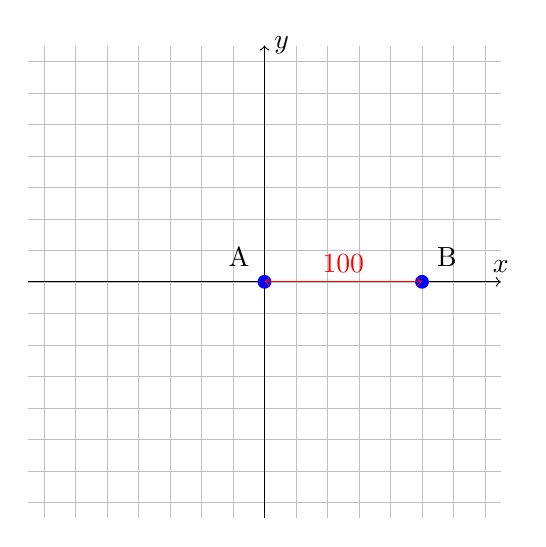
\begin{tikzpicture}[scale=0.02]
        \draw[lightgray,very thin,step=20] (-150,-150) grid (150,150);
        \draw[->] (-150,0)--(150,0) node[above]{$x$};
        \draw[->] (0,-150)--(0,150) node[right]{$y$};
        \node[shape=circle,fill=blue,minimum size=5pt,inner sep=1pt,label=135:A] at (0,0) {};
        \node[shape=circle,fill=blue,minimum size=5pt,inner sep=1pt,label=45:B] at (100,0) {};
        \draw[color=red,<->] (0,0)--(100,0) node[midway,above]{$100$};
      \end{tikzpicture}
      &
      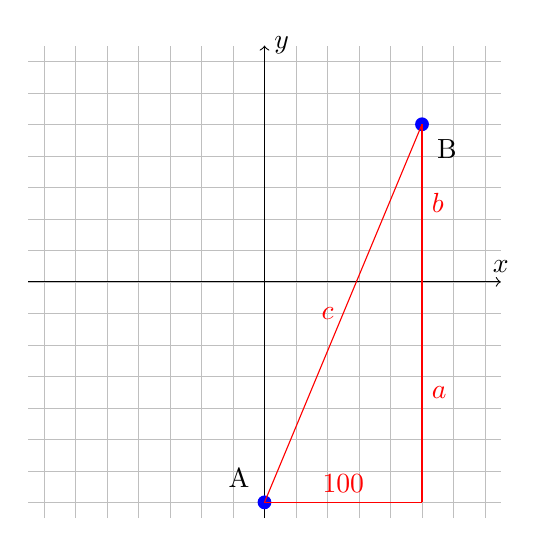
\begin{tikzpicture}[scale=0.02]
        \draw[lightgray,very thin,step=20] (-150,-150) grid (150,150);
        \draw[->] (-150,0)--(150,0) node[above]{$x$};
        \draw[->] (0,-150)--(0,150) node[right]{$y$};
        \node[shape=circle,fill=blue,minimum size=5pt,inner sep=1pt,label=135:A] at (0,-140) {};
        \node[shape=circle,fill=blue,minimum size=5pt,inner sep=1pt,label=315:B] at (100,100) {};
        \draw[color=red] (0,-140)--(100,-140) node[midway,above]{$100$};
        \draw[color=red] (100,-140)--(100,0) node[midway,right]{$a$};
        \draw[color=red] (100,0)--(100,100) node[midway,right]{$b$};
        \draw[color=red] (0,-140)--(100,100) node[midway,left]{$c$};
      \end{tikzpicture}
      \\
      \mbox{(a) Buses at noon}
      &
      \mbox{(b) Buses at 2 pm}
    \end{array}$
    \caption{Diagrams for problem~\ref{prob:bus}}
    \label{fig:bus}
  \end{figure}
  To find the rate at which the buses are moving apart from
  one another, we use related rates.  Let the position of the bus departing
  from $A$ at time $t$ be $a(t)$ units below its starting point,
  and let the position of the bus departing
  from $B$ at time $t$ be $b(t)$ units above its starting point.  
  Let $c(t)$ be the distance between
  the buses.  By the Pythagorean Theorem we have
  \begin{equation*}
    (c(t))^2 = 100^2 + (a(t)+b(t))^2
  \end{equation*}
  Differentiating with respect to $t$,
  \begin{equation*}
    2c\frac{dc}{dt} = 0 + 2(a+b)\left(\frac{da}{dt}+\frac{db}{dt}\right)
  \end{equation*}
  From the above information, at $t=2$ we have $a=140$, $b=100$, $c=260$,
  $da/dt=70$, and $db/dt=50$.  Putting all that into the above equation
  gives
  \begin{equation*}
    2(260) \frac{dc}{dt} = 2(140+100) \left( 70+50\right)
    \implies \frac{dc}{dt} = \frac{240\cdot 120}{260} \approx 111
  \end{equation*}
  The buses are moving away from one another at a rate of approximately
  $111$ kilometers per hour.
\item\label{prob:graph} %7
  \begin{enumerate}
  \item %7a
    We find the $y$-intercept by setting $x=0$:
    \begin{equation*}
      f(0)= \frac{2-0}{\sqrt{0^2+2}} = \frac{2}{\sqrt{2}} = \sqrt{2}
    \end{equation*}
    We find the $x$-intercepts by setting $y=0$, i.e. by solving the equation
    \begin{equation*}
      f(x)=0 \implies \frac{2-x}{\sqrt{x^2+2}} = 0 \implies 2-x = 0 \implies
      x=2
    \end{equation*}

    The local maxima and minima are at critical numbers, which we find
    by solving the equation
    \begin{equation*}
      f'(x) = 0 \implies \frac{-2x-2}{(x^2+2)^{3/2}} = 0
      \implies -2x-2=0 \implies x=-1
    \end{equation*}
    We could determine whether we have a local max or min at $x=-1$ using
    the First Derivative Test, but we leave that for part (b).  Instead,
    because the second derivative of $f$ has already been calculated, it may
    be easier to use the second derivative test:
    \begin{equation*}
      f''(-1) = \frac{2(-1+2)(2(-1)-1)}{((-1)^2+2)^{5/2}}
      = \frac{2(1)(-3)}{(1+2)^{5/2}} < 0
    \end{equation*}
    so by the second derivative test there is a local maximum at $x=-1$, and
    no local minimum.

    To find potential inflection numbers we solve the equation
    \begin{equation*}
      f''(x)=0 \implies \frac{2(x+2)(2x-1)}{(x^2+2)^{5/2}} = 0
      \implies 2(x+2)(2x-1)=0
      \implies \mbox{$x=-2$ or $x=1/2$}
    \end{equation*}
    We will see below in part~(b) that the sign of $f''$ changes across each
    of the potential inflection numbers, so they are both actual inflection
    numbers.

    Finally, there are potential vertical asymptotes 
    where $f(x)$ is undefined,
    which is where the denominator is zero, i.e.,
    $\sqrt{x^2+2}=0$ or where the expression
    under the square root is negative, i.e., $x^2+2<0$.  
    Since $x^2\ge 0$, we have
    $x^2+2\ge 2 > 0$ so neither of the above cases is possible, $f(x)$ is
    defined everywhere, and it has no vertical asymptotes.  
    Horizontal asymptotes are found by evaluating the limits at infinity
    \begin{equation*}
      \mbox{$\ds\lim_{x\to\infty} f(x)$ and $\ds\lim_{x\to -\infty} f(x)$}
    \end{equation*}
    In the first case we divide through by the highest power of $x$ in
    the denominator, namely $\sqrt{x^2}$, to obtain
    \begin{equation*}
      \lim_{x\to\infty} \frac{2-x}{\sqrt{x^2+2}}
      = \lim_{x\to\infty} \frac{2-x}{\sqrt{x^2+2}}
        \cdot \frac{1/x}{1/\sqrt{x^2}}
      = \lim_{x\to\infty} \frac{2/x-1}{\sqrt{1+2/x^2}}
      = \frac{0-1}{\sqrt{1+0}} = -1
    \end{equation*}
    so there is a horizontal asymptote at $y=-1$.  On the other hand, as
    $x\to -\infty$, $x$ is negative, so $\sqrt{x^2}=-x$ and we have
    \begin{equation*}
      \lim_{x\to -\infty} \frac{2-x}{\sqrt{x^2+2}}
      = \lim_{x\to -\infty} \frac{2-x}{\sqrt{x^2+2}}
        \cdot -\frac{1/x}{1/\sqrt{x^2}}
      = -\lim_{x\to -\infty} \frac{2/x-1}{\sqrt{1+2/x^2}}
      = -\frac{0-1}{\sqrt{1+0}} = 1
    \end{equation*}
    so $y=1$ is another horizontal asymptote.
  \item %7b
    To determine intervals of increase/decrease, we split the $x$ axis up
    at the critical numbers and create Table~\ref{tab:crit}.  Note that
    the denominator $(x^2+2)^{3/2}$ is always positive so it doesn't 
    affect the sign of $f'(x)$.
    \begin{table}[htbp]
      \centering
      \begin{tabular}{|c|c|c|c|c|}
        \hline
        Interval       & $-2$ & $x+1$ & $f'(x)$ & $f(x)$ 
        \\ \hline
        $-\infty<x<-1$ & $-$  & $-$   & $+$     & increasing 
        \\ \hline
        $x=-1$         & $-$  & $0$   & $0$     & stationary
        \\ \hline
        $-1<x<\infty$  & $-$  & $+$   & $-$     & decreasing
        \\ \hline
      \end{tabular}
      \caption{Intervals of increase/decrease for problem~\ref{prob:graph}}
      \label{tab:crit}
    \end{table}
    From the table we see that $f(x)$ is increasing on $(-\infty,-1)$ and
    decreasing on $(-1,\infty)$, and by the First Derivative Test
    we verify that $x=-1$ is a local maximum for $f$.

    To determine intervals of concavity we create a similar table for $f''$.
    See Table~\ref{tab:conc}.
    Again note that $(x^2+2)^{5/2}$ is always positive so it doesn't
    affect the sign of $f''$.
    \begin{table}[htbp]
      \centering
      \begin{tabular}{|c|c|c|c|c|}
        \hline
        Interval       & $x+2$ & $x-1/2$ & $f''(x)$ & $f(x)$ 
        \\ \hline
        $-\infty<x<-2$ & $-$   & $-$     & $+$      & concave up 
        \\ \hline
        $x=-2$         & $0$   & $-$     & $0$      & inflection
        \\ \hline
        $-2<x<1/2$     & $+$   & $-$     & $-$      & concave dn 
        \\ \hline
        $x=1/2$        & $+$   & $0$     & $0$      & inflection
        \\ \hline
        $1/2<x<\infty$ & $+$   & $+$     & $+$      & concave up
        \\ \hline
      \end{tabular}
      \caption{Intervals of concavity for problem~\ref{prob:graph}}
      \label{tab:conc}
    \end{table}
    From the table we see that $f$ is concave up on $(-\infty,-2)$ and
    $(1/2,\infty)$, and concave down on $(-2,1/2)$.  Since the concavity
    changes across both potential inflection points $x=-2$ and $x=1/2$,
    they are both actual inflection points, as mentioned above in~(a).
  \item %7c
    We calculate the $y$ values of all the interesting points on the graph.
    We have the intercepts $(0,\sqrt{2})$, $(2,0)$, and the local maximum
    and inflection points:
    \begin{align*}
      x=-1 &\implies y=f(-1)=\frac{2-(-1)}{\sqrt{(-1)^2+2}} = \sqrt{3}
      \\
      x=-2 &\implies y=f(-2)= \frac{2-(-2)}{\sqrt{(-2)^2+2}} 
      = \frac{2\sqrt{6}}{3}
      \\
      x=1/2 &\implies y=f(1/2) = \frac{2-1/2}{\sqrt{(1/2)^2+2}}
      = \frac{3}{\sqrt{1+2(2)^2}} = 1
    \end{align*}
    In addition to those five points, we plot the asymptotes on the graph,
    one to the left of the $y$-axis and one to the right of the $y$-axis.
    We obtain Figure~\ref{fig:graph}(a).  Then we join the points with 
    appropriate arcs which are increasing or decreasing, concave up or down,
    and framed by asymptotes as determined by the results of part~(b).
    For the final graph, see Figure~\ref{fig:graph}(b).
    \begin{figure}[htbp]
      \centering
      $\begin{array}{c@{\hspace{0.05in}}c}
        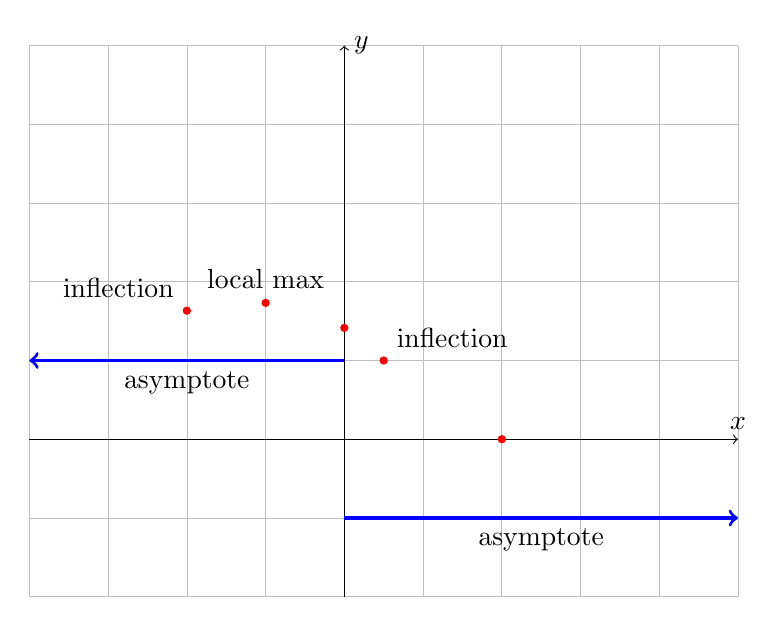
\begin{tikzpicture}
          \draw[lightgray,very thin] (-4,-2) grid (5,5);
          \draw[->] (-4,0)--(5,0) node[above]{$x$};
          \draw[->] (0,-2)--(0,5) node[right]{$y$};
          \path
            let
              \p{i1} = (0,{sqrt(2)}),
              \p{i2} = (2,0),
              \p{m1} = (-1,{sqrt(3)}),
              \p{f1} = (-2,{sqrt(24/9)}),
              \p{f2} = (0.5,1)
            in
              coordinate (i1) at (\p{i1})
              coordinate (i2) at (\p{i2})
              coordinate (m1) at (\p{m1})
              coordinate (f1) at (\p{f1})
              coordinate (f2) at (\p{f2});
          \node[fill=red,shape=circle,minimum size=3pt,inner sep=1pt] at (i1){};
          \node[fill=red,shape=circle,minimum size=3pt,inner sep=1pt] at (i2){};
          \node[fill=red,shape=circle,minimum size=3pt,inner sep=1pt,label=above:local max] at (m1){};
          \node[fill=red,shape=circle,minimum size=3pt,inner sep=1pt,label=135:inflection] at (f1){};
          \node[fill=red,shape=circle,minimum size=3pt,inner sep=1pt,label=45:inflection] at (f2){};
          \draw[color=blue,very thick,<-] (-4,1)--(0,1) 
            node[color=black,midway,below]{asymptote};
          \draw[color=blue,very thick,->] (0,-1)--(5,-1)
            node[color=black,midway,below]{asymptote};
        \end{tikzpicture}
        &
        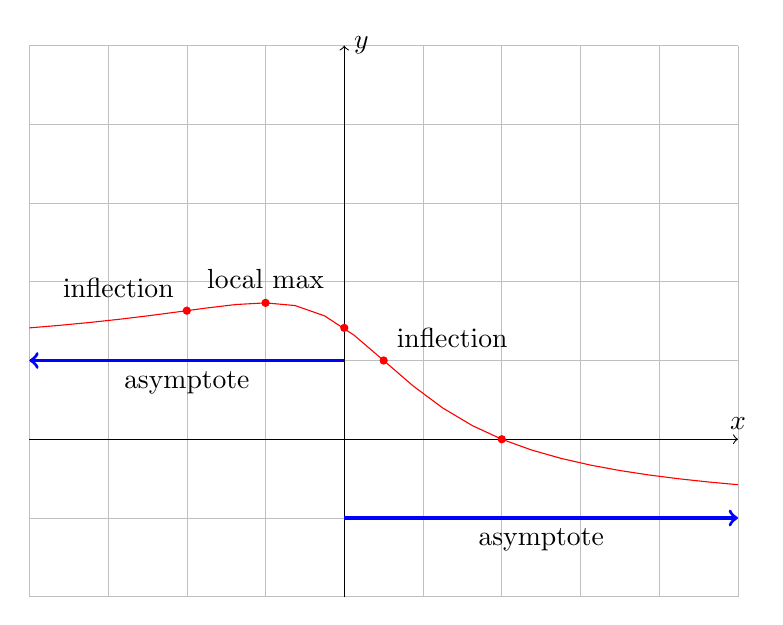
\begin{tikzpicture}
          \draw[lightgray,very thin] (-4,-2) grid (5,5);
          \draw[->] (-4,0)--(5,0) node[above]{$x$};
          \draw[->] (0,-2)--(0,5) node[right]{$y$};
          \draw[color=red,domain=-4:5] plot (\x,{(2-\x)/sqrt((\x)^2+2)});
          \path
            let
              \p{i1} = (0,{sqrt(2)}),
              \p{i2} = (2,0),
              \p{m1} = (-1,{sqrt(3)}),
              \p{f1} = (-2,{sqrt(24/9)}),
              \p{f2} = (0.5,1)
            in
              coordinate (i1) at (\p{i1})
              coordinate (i2) at (\p{i2})
              coordinate (m1) at (\p{m1})
              coordinate (f1) at (\p{f1})
              coordinate (f2) at (\p{f2});
          \node[fill=red,shape=circle,minimum size=3pt,inner sep=1pt] at (i1){};
          \node[fill=red,shape=circle,minimum size=3pt,inner sep=1pt] at (i2){};
          \node[fill=red,shape=circle,minimum size=3pt,inner sep=1pt,label=above:local max] at (m1){};
          \node[fill=red,shape=circle,minimum size=3pt,inner sep=1pt,label=135:inflection] at (f1){};
          \node[fill=red,shape=circle,minimum size=3pt,inner sep=1pt,label=45:inflection] at (f2){};
          \draw[color=blue,very thick,<-] (-4,1)--(0,1)
            node[color=black,midway,below]{asymptote};
          \draw[color=blue,very thick,->] (0,-1)--(5,-1)
            node[color=black,midway,below]{asymptote};
        \end{tikzpicture}
        \\
        \mbox{(a) Points and lines} 
        &
        \mbox{(b) Arcs; completed graph}
      \end{array}$
      \caption{Graph of $y=(2-x)/\sqrt{x^2+2}$ for problem~\ref{prob:graph}}
      \label{fig:graph}
    \end{figure}
  \end{enumerate}
\item\label{prob:fence} %8
  Let one of the sides of the rectangle
  have length $x$ and the other have length $y$.
  See Figure~\ref{fig:fence}.
  \begin{figure}[htbp]
    \centering
    \begin{tikzpicture}[scale=0.5]
      \draw (0,0) --
        node[midway,below]{$y$} 
        (50/2,0)--(50/2,50/7)--(0,50/7)--
        node[midway,left]{$x$}
        (0,0);
      \foreach \n in {1,2,3,4,5} {
        \draw ({25/6*\n},0)--({25/6*\n},50/7);
      }
    \end{tikzpicture}
    \caption{Diagram for problem~\ref{prob:fence}}
    \label{fig:fence}
  \end{figure}
  Assume the five interior fences are parallel to the side of length $x$.
  Then the total amount of fencing used is $2x+2y$ for the outside perimeter,
  $5x$ for the inside fence, for a total of $7x+2y$ feet of fence.  Since
  we have $100$ feet available, we have the constraint $7x+2y=100$.  The
  total area is $A=xy$.  Solving for $y$ in the constraint and substituting
  it into the objective we have
  \begin{equation*}
    2y=100-7x \implies y = 50-\frac{7}{2} x
    \implies A = x\left(50-\frac{7}{2} x\right) = 50x-\frac{7}{2}x^2
  \end{equation*}
  Differentiating, $A'(x)= 50-7x$.  The critical number is where $A'(x)=0$, 
  i.e., $x=50/7$.  By inspection (or by drawing up a table as in 
  problem~\ref{prob:graph}), we see that $A'(x)>0$ for $x<7$ and $A'(x)<0$
  for $x>7$, so $A(x)$ has a global maximum at $x=50/7$.  Therefore the
  dimensions of the enclosure that maximize the area are $x=50/7\approx 7.1$ 
  feet and $y=50-(7/2)(50/7) = 25$ feet.
\item\label{prob:area} %9
  First sketch a graph of the region in question.  There is one bounded
  region defined by the two curves. 
  \begin{figure}[htbp]
    \centering
    $\begin{array}{c@{\hspace{0.5in}}c}
    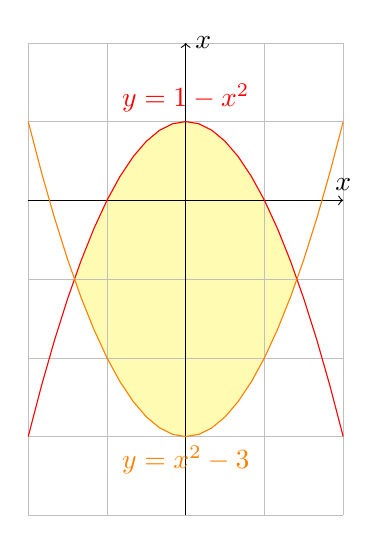
\begin{tikzpicture}
      \fill[color=yellow!30!white,domain=-1.4142:1.4142] plot (\x,{1-(\x)^2}) -- plot (\x,{(\x)^2-3}) --cycle;
      \draw[lightgray,very thin] (-2,-4) grid (2,2);
      \draw[->] (-2,0)--(2,0) node[above]{$x$};
      \draw[->] (0,-4)--(0,2) node[right]{$x$};
      \draw[color=red,domain=-2:2] plot (\x,{1-(\x)^2});
      \draw  node[above,color=red] at (0,1) {$y=1-x^2$};
      \draw[color=orange,domain=-2:2] plot (\x,{(\x)^2-3}) ;
      \draw  node[below,color=orange] at (0,-3) {$y=x^2-3$};
    \end{tikzpicture}
    &
    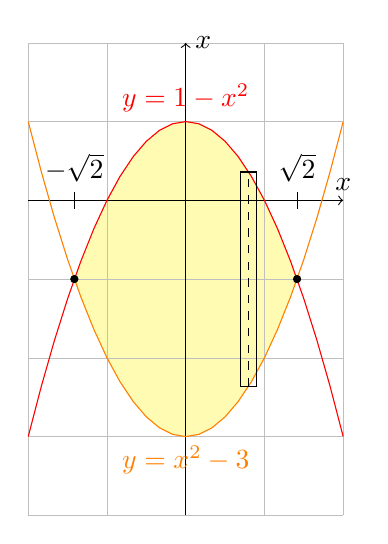
\begin{tikzpicture}
      \fill[color=yellow!30!white,domain=-1.4142:1.4142] plot (\x,{1-(\x)^2}) -- plot (\x,{(\x)^2-3}) --cycle;
      \draw[lightgray,very thin] (-2,-4) grid (2,2);
      \draw[->] (-2,0)--(2,0) node[above]{$x$};
      \draw[->] (0,-4)--(0,2) node[right]{$x$};
      \draw (-1.4142,-3pt)--(-1.4142,3pt) node[above]{$-\sqrt{2}$};
      \draw (1.4142,-3pt)--(1.4142,3pt) node[above]{$\sqrt{2}$};
      \draw[color=red,domain=-2:2] plot (\x,{1-(\x)^2});
      \draw  node[above,color=red] at (0,1) {$y=1-x^2$};
      \draw[color=orange,domain=-2:2] plot (\x,{(\x)^2-3}) ;
      \draw  node[below,color=orange] at (0,-3) {$y=x^2-3$};
      \node[fill=black,shape=circle,minimum size=3pt,inner sep=1pt] 
        at (-1.4142,-1) {};
      \node[fill=black,shape=circle,minimum size=3pt,inner sep=1pt] 
        at (1.4142,-1) {};
      \path
        let
          \n{r0}  = {0.7},
          \n{r1}  = {0.8},
          \n{r2}  = {0.9},
          \p{r00} = (\n{r0},{(\n{r1})^2-3}),
          \p{r01} = (\n{r1},{(\n{r1})^2-3}),
          \p{r02} = (\n{r2},{(\n{r1})^2-3}),
          \p{r10} = (\n{r0},{1-(\n{r1})^2}),
          \p{r11} = (\n{r1},{1-(\n{r1})^2}),
          \p{r12} = (\n{r2},{1-(\n{r1})^2})
        in
          coordinate (r00) at (\p{r00})
          coordinate (r01) at (\p{r01})
          coordinate (r02) at (\p{r02})
          coordinate (r10) at (\p{r10})
          coordinate (r11) at (\p{r11})
          coordinate (r12) at (\p{r12});
      \draw[color=black] (r00)--(r02)--(r12)--(r10)--cycle;
      \draw[color=black,dashed] (r01)--(r11);
    \end{tikzpicture}
    \end{array}$
    \caption{Graphs for problem~\ref{prob:area}}
    \label{fig:area}
  \end{figure}
  We then find the endpoints of the bounded region
  by finding intersection points of the curves:
  \begin{equation*}
    1-x^2 = x^2-3 \implies 2x^2=4 \implies x=\pm \sqrt{2}
  \end{equation*}
  and we add to the graph a typical rectangle for the Riemann sum for the
  area, with width $dx$ and height equal to the difference between the 
  functions from the higher curve to the lower curve at some point $x_i^*$
  inside the rectangle.
  Now we set up the integral for the area.  It is the integral of the
  upper curve minus the lower curve, with bounds determined by the 
  intersection points of the curves:
  \begin{multline*}
    A = \int_{-\sqrt{2}}^{\sqrt{2}} \left( (1-x^2) - (x^2-3)\right) \; dx
    = \int_{-\sqrt{2}}^{\sqrt{2}} (4-2x^2) \; dx
    = \left. \vphantom{\int} \left( 4x-\frac{2}{3} x^3 \right) 
    \right|_{-\sqrt{2}}^{\sqrt{2}}
    \\
    = (\sqrt{2}) \left(4-\frac{2}{3}(\sqrt{2})^2\right)
    - (-\sqrt{2}) \left(4-\frac{2}{3}(-\sqrt{2})^2\right)
    = 2\sqrt{2} \left( 4-\frac{4}{3}\right)
    = \frac{16\sqrt{2}}{3}
  \end{multline*}
\item %10
  \begin{enumerate}
  \item %a
    Writing in power notation and performing algebraic simplifications,
    \begin{equation*}
      \int \frac{x+2x^{1/2} +1}{x^{1/2}} \; dx
      = \int \left( x^{1/2} + 2 + x^{-1/2} \right) \; dx
      = \frac{x^{3/2}}{3/2} + 2x + \frac{x^{1/2}}{1/2} + C
      = \frac{2}{3} x^{3/2} + 2x + 2 x^{1/2} + C
    \end{equation*}
    You should check by differentiating.
  \item %b
    First we do the indefinite integral.  Let $u=2\pi t^2$, 
    $du = 4\pi t \; dt$, $du/(4\pi) = t\; dt$:
    \begin{equation*}
      \int t \sin (2\pi t^2) \; dt
      = \frac{1}{4\pi} \int \sin u \; du
      = -\frac{1}{4\pi} \cos u + C
      = -\frac{1}{4\pi} \cos (2\pi t^2) + C
    \end{equation*}
    You should check the above result by differentiating.  Now we can
    evaluate the definite integral by the Fundamental Theorem of Calculus:
    \begin{multline*} 
      \int_0^{1/2} t\sin (2\pi t^2) \; dt
      = \left. \int t\sin(2\pi t^2) \; dt \right|_{0}^{1/2}
      = \left. \vphantom{\int} -\frac{1}{4\pi} \cos (2\pi t^2) \right|_0^{1/2}
      \\
      = -\frac{1}{4\pi} \cos (2\pi(1/2)^2) 
      + \frac{1}{4\pi} \cos (2\pi(0)^2)
      = -\frac{1}{4\pi} \cos(\pi/2) + \frac{1}{4\pi} \cos(0)
      = \frac{1}{4\pi}
    \end{multline*}
  \item %c
    Let $u=\theta^{1/2}$, $du = (1/2) \theta^{-1/2} \; d\theta$,
    $2du = \theta^{-1/2} \; d\theta$:
    \begin{equation*}
      \int \cos(\theta^{1/2}) \cdot \theta^{-1/2} \; d\theta
      = 2 \int \cos u \; du
      = 2 \sin u + C
      = 2 \sin(\theta^{1/2}) + C
    \end{equation*}
    Check by differentiating.
  \item %d
    For variety, let's use the second method for a substitution in a 
    definite integral.  Let $u=1-x^2$, $du=-2x \;dx$, $-du/2=x\; dx$;
    when $x=0$, $u=1$, and when $x=1$, $u=0$.  We have
    \begin{equation*}
      \int_0^1 x \sqrt{1-x^2} \; dx
      = -\frac{1}{2} \int_1^0 u^{1/2} \; du
      = \frac{1}{2} \int_0^1 u^{1/2} \; du
      = \left. \vphantom{\int} \frac{1}{2} \frac{u^{3/2}}{3/2} \right|_{0}^1
      = \frac{1}{3} (1^{3/2}-0^{3/2}) = \frac{1}{3}
    \end{equation*}
  \end{enumerate}
\end{enumerate}


\end{document}

